%
% teil2.tex -- Beispiel-File für teil2 
%
% (c) 2020 Prof Dr Andreas Müller, Hochschule Rapperswil
%
\section{Fraktale mit IFS 
\label{ifs:section:teil2}}
\rhead{Teil 2}
Wollen wir nun eine bestimmte Art anschauen, wie man Fraktale machen kann.
Zur Veranschaulichung dieser Methode nehmen wir das Sierpinski Dreieck.
\begin{figure}
	\label{ifs:sierpinski10}
	\centering
	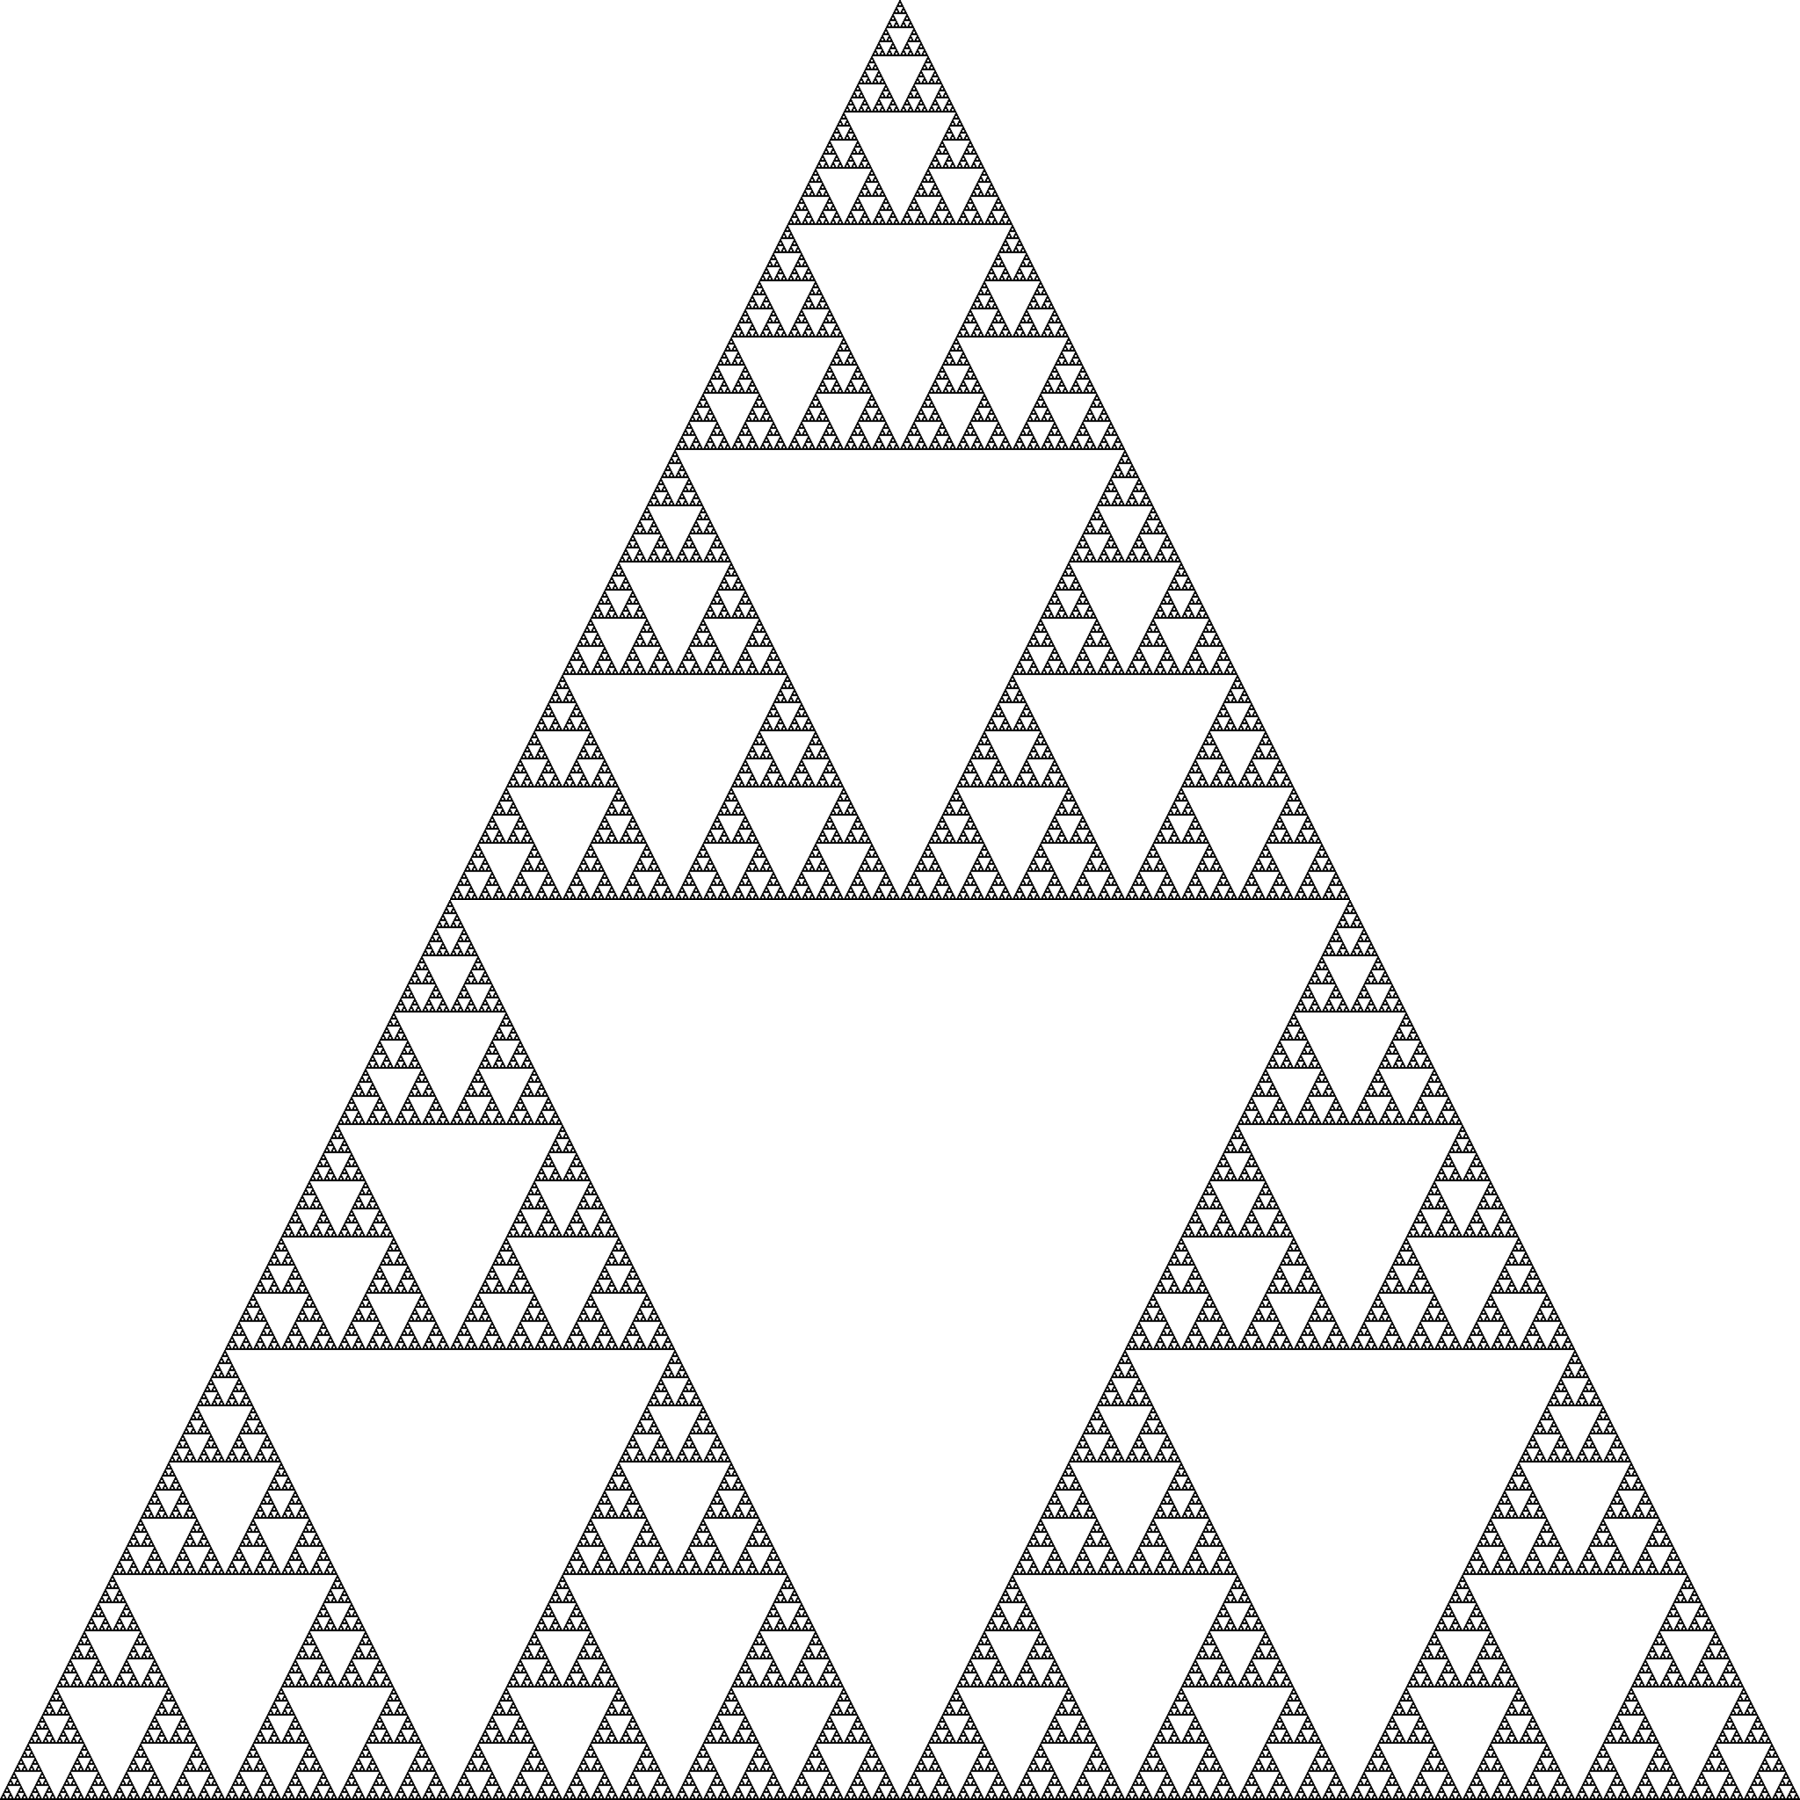
\includegraphics[width=0.5\textwidth]{papers/ifs/images/sierpinski}
	\caption{Sierpinski-Dreieck}
\end{figure}
Wenn man das Dreieck genau anschaut, erkennt man schnell, dass es aus drei kleineren Kopien seiner selbst besteht.
Es ist also ein Selbstähnliches Konstrukt.
Diese Eigenschaft wollen wir uns zunutze machen.


Wir definieren das Dreieck mit Kantenlänge 1 als Menge $X$.
Ausserdem bestimmen wir drei Funktionen, welche die gesamte Menge auf eine ihrer kleineren Kopien abbildet
\begin{align*}
	f_1(x,y)
	= 
	\begin{pmatrix}
		\frac{1}{2} & 0 \\
		0 & \frac{1}{2} \\
	\end{pmatrix}
	\begin{pmatrix}
		x\\
		y\\
	\end{pmatrix} 
	,\quad
	f_2(x,y)
	= 
	\begin{pmatrix}
		\frac{1}{2} & 0 \\
		0 & \frac{1}{2} \\
	\end{pmatrix}
	\begin{pmatrix}
		x\\
		y\\
	\end{pmatrix} 
	+
	\begin{pmatrix}
		\frac{1}{2} \\
		0
	\end{pmatrix}
	, \quad
	f_3(x,y)
	= 
	\begin{pmatrix}
		\frac{1}{2} & 0 \\
		0 & \frac{1}{2} \\
	\end{pmatrix}
	\begin{pmatrix}
		x\\
		y\\
	\end{pmatrix} 
	+
	\begin{pmatrix}
		\frac{1}{4} \\
		\frac{1}{2}
	\end{pmatrix}\\
\end{align*}
$f_1$ bildet das Dreieck auf das Teilstück unten links ab, $f_2$ auf das Teilstück unten rechts und $f_3$ auf das obere Teilstück.
Wendet man alle drei Funktionen auf das Sierpinski-Dreieck an, entsteht also wieder ein Sierpinski-Dreieck.
\begin{align*}
	X = \bigcup\limits_{i = 1}^{3} f_i(X)
\end{align*}
Man kann sogar noch einen Schritt weiter gehen, und sagen: Wenn wir die Funktionen auf eine beliebige Startmenge anwenden, konvergiert die Menge gegen das Sierpinski-Dreieck.
\begin{figure}
	\label{ifs:sierpconst}
	\centering
	\subfigure[]{
		\label{ifs:sierpconsta}
		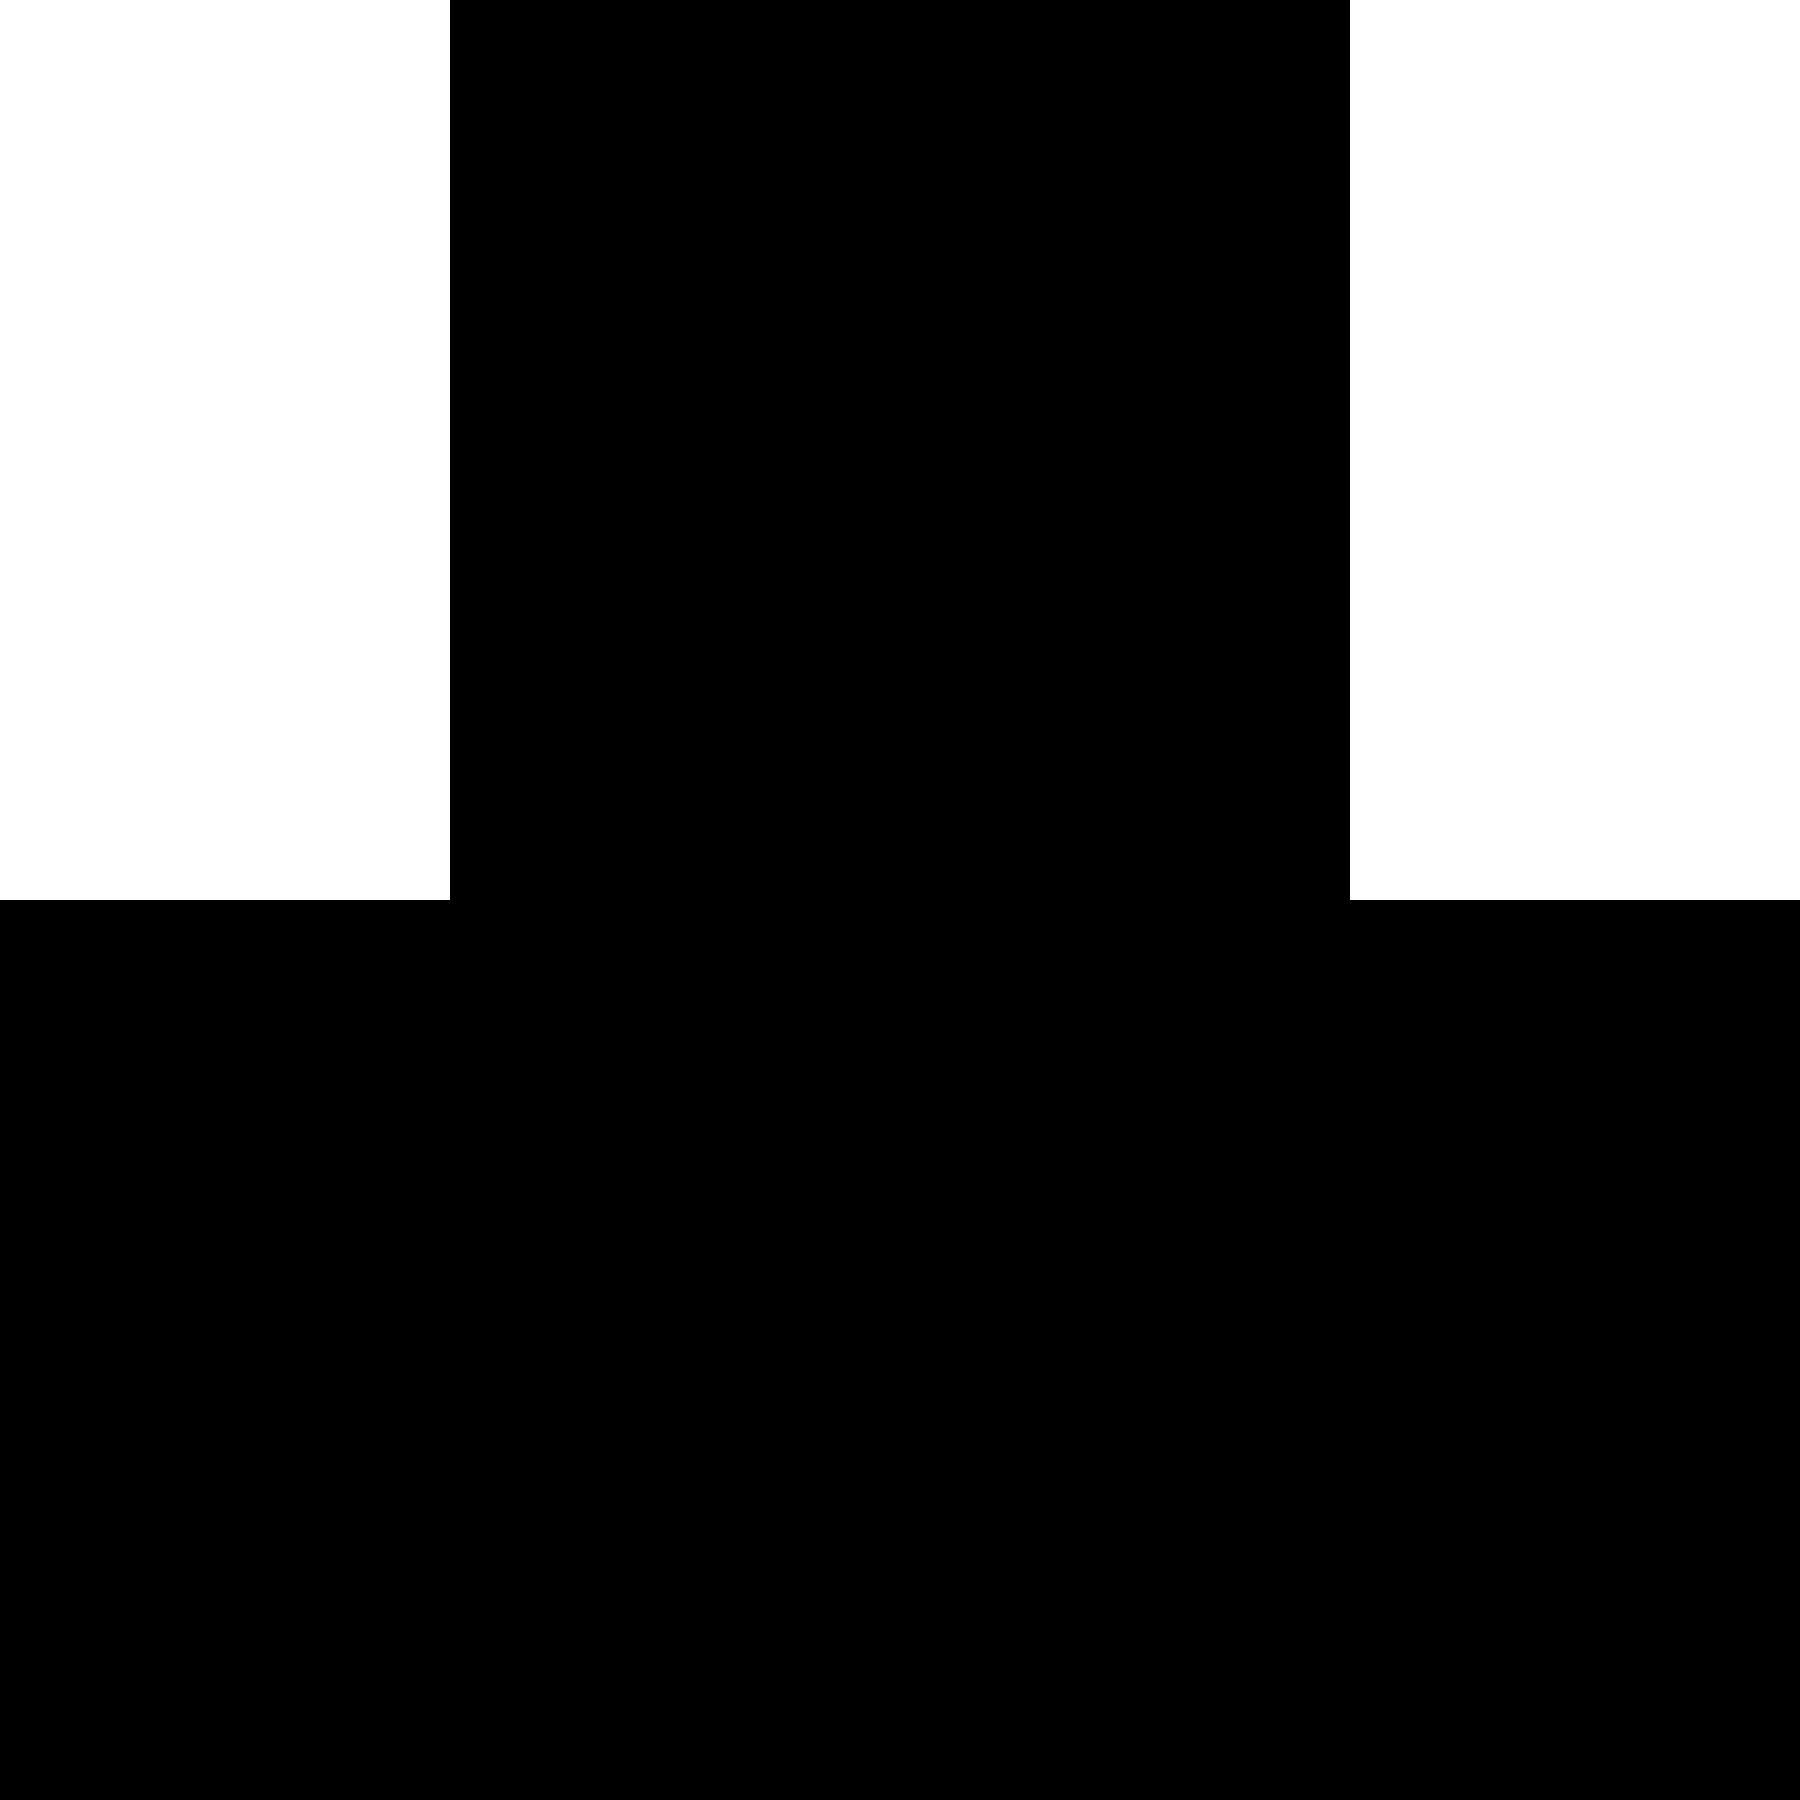
\includegraphics[width=0.25\textwidth]{papers/ifs/images/sierpinski1}}
	\subfigure[]{
		\label{ifs:sierpconstb}
		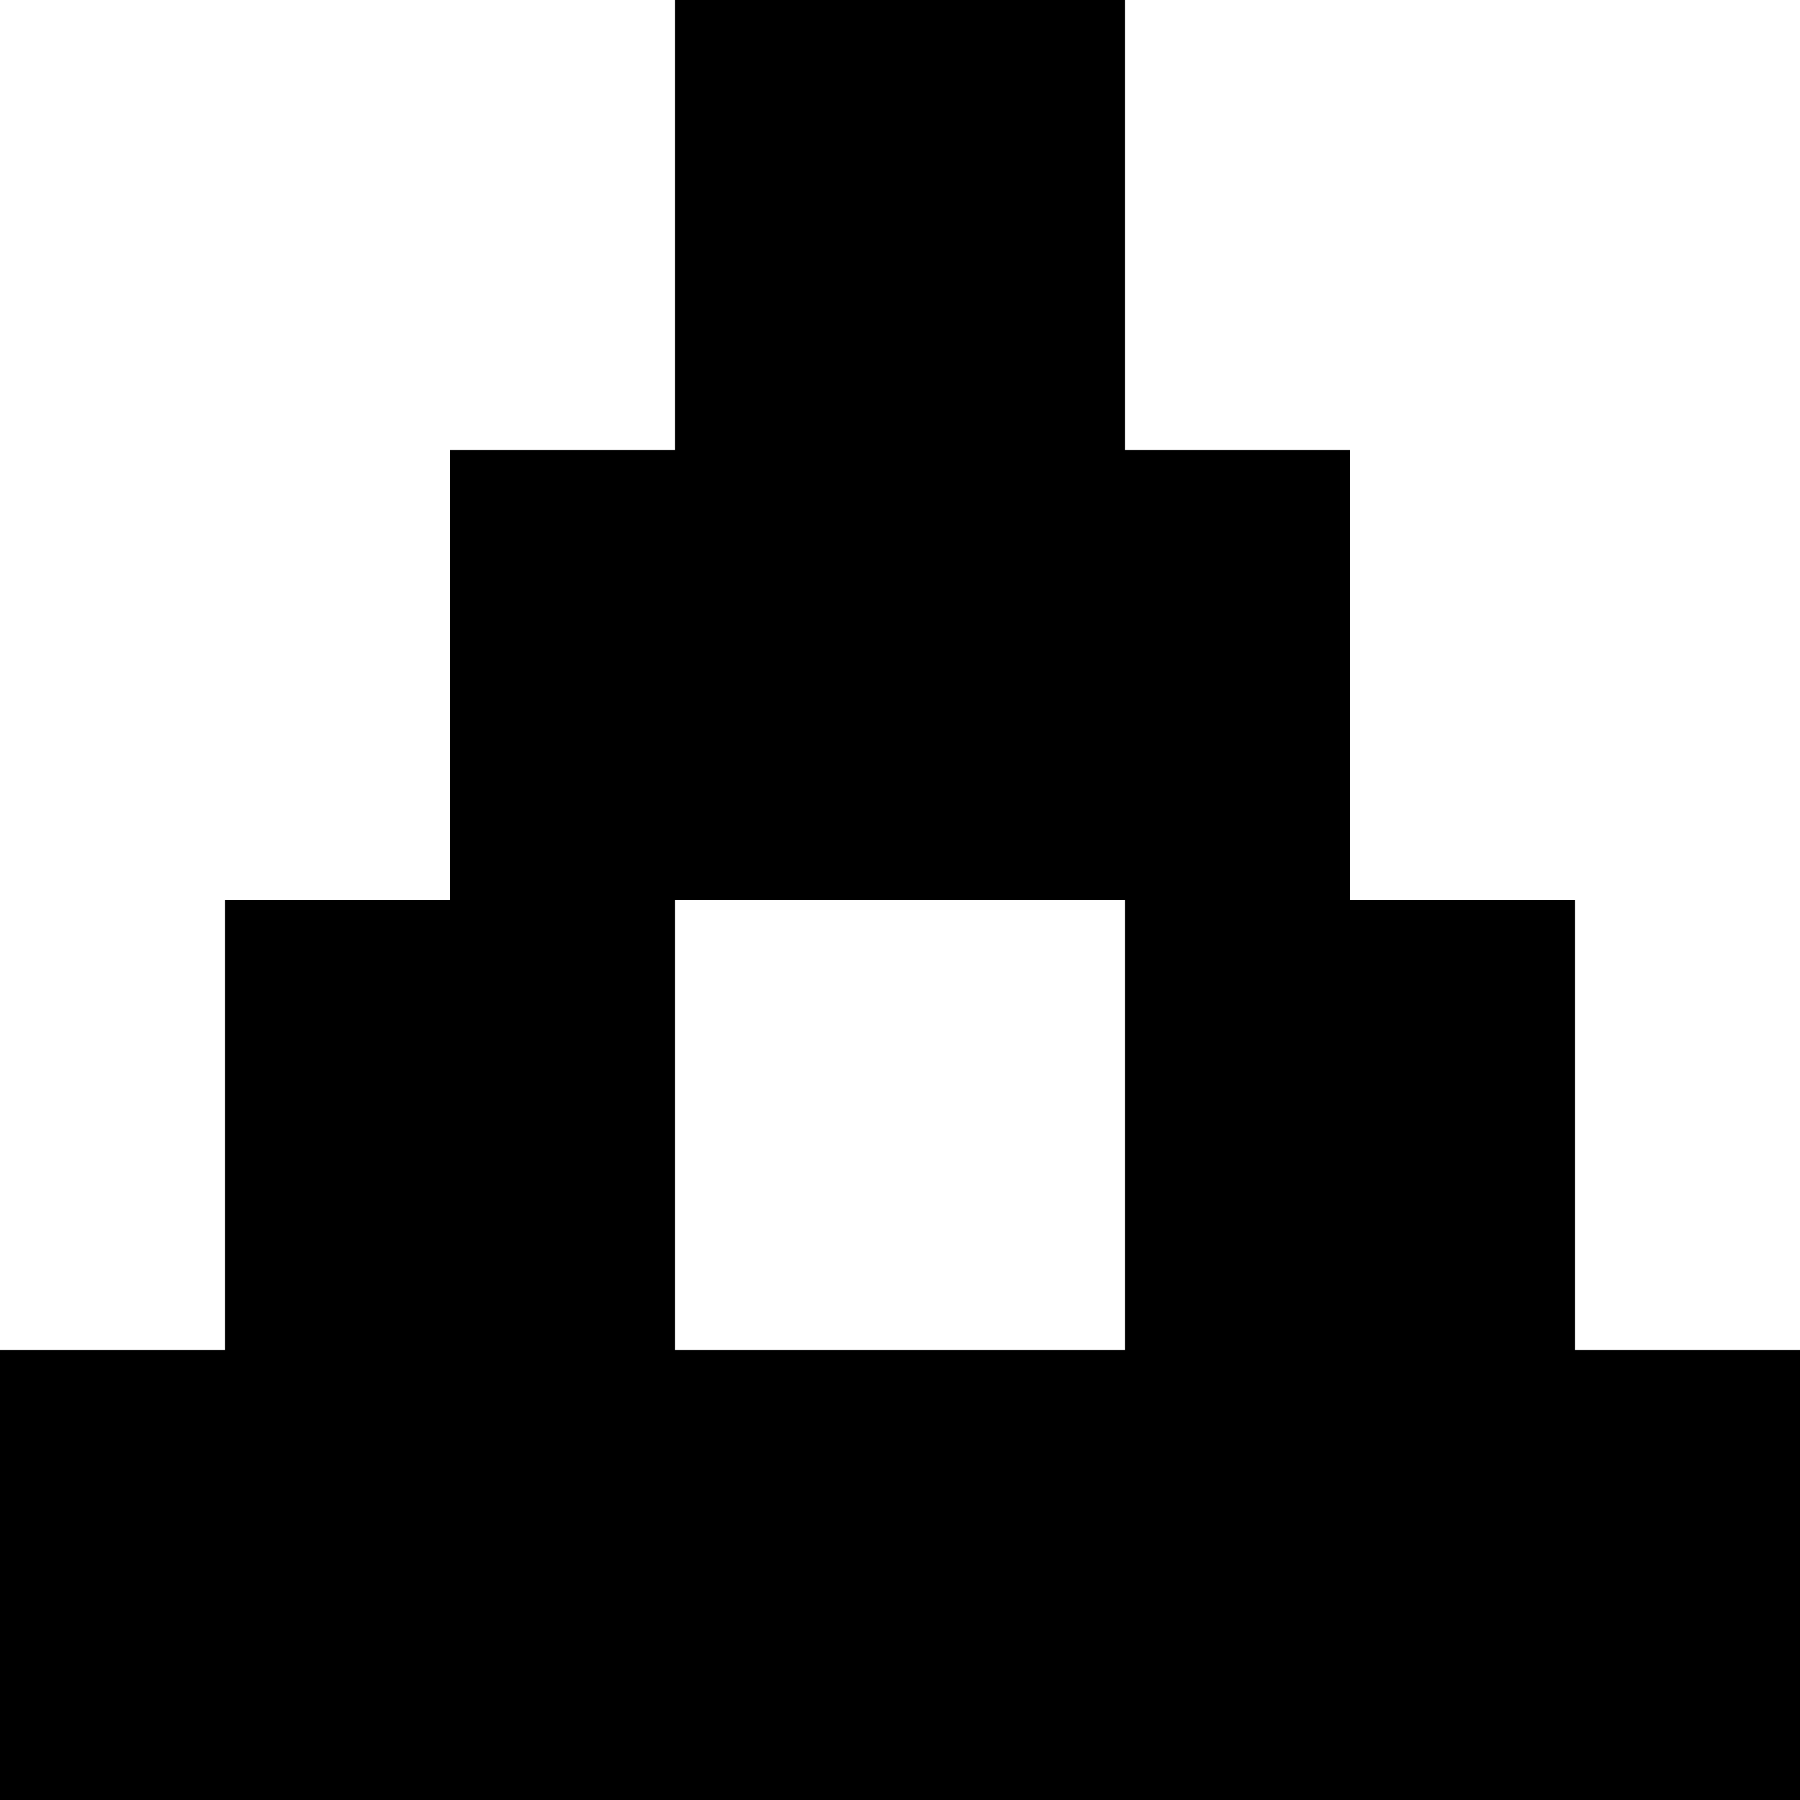
\includegraphics[width=0.25\textwidth]{papers/ifs/images/sierpinski2}} 
	\subfigure[]{
		\label{ifs:sierpconstc}
		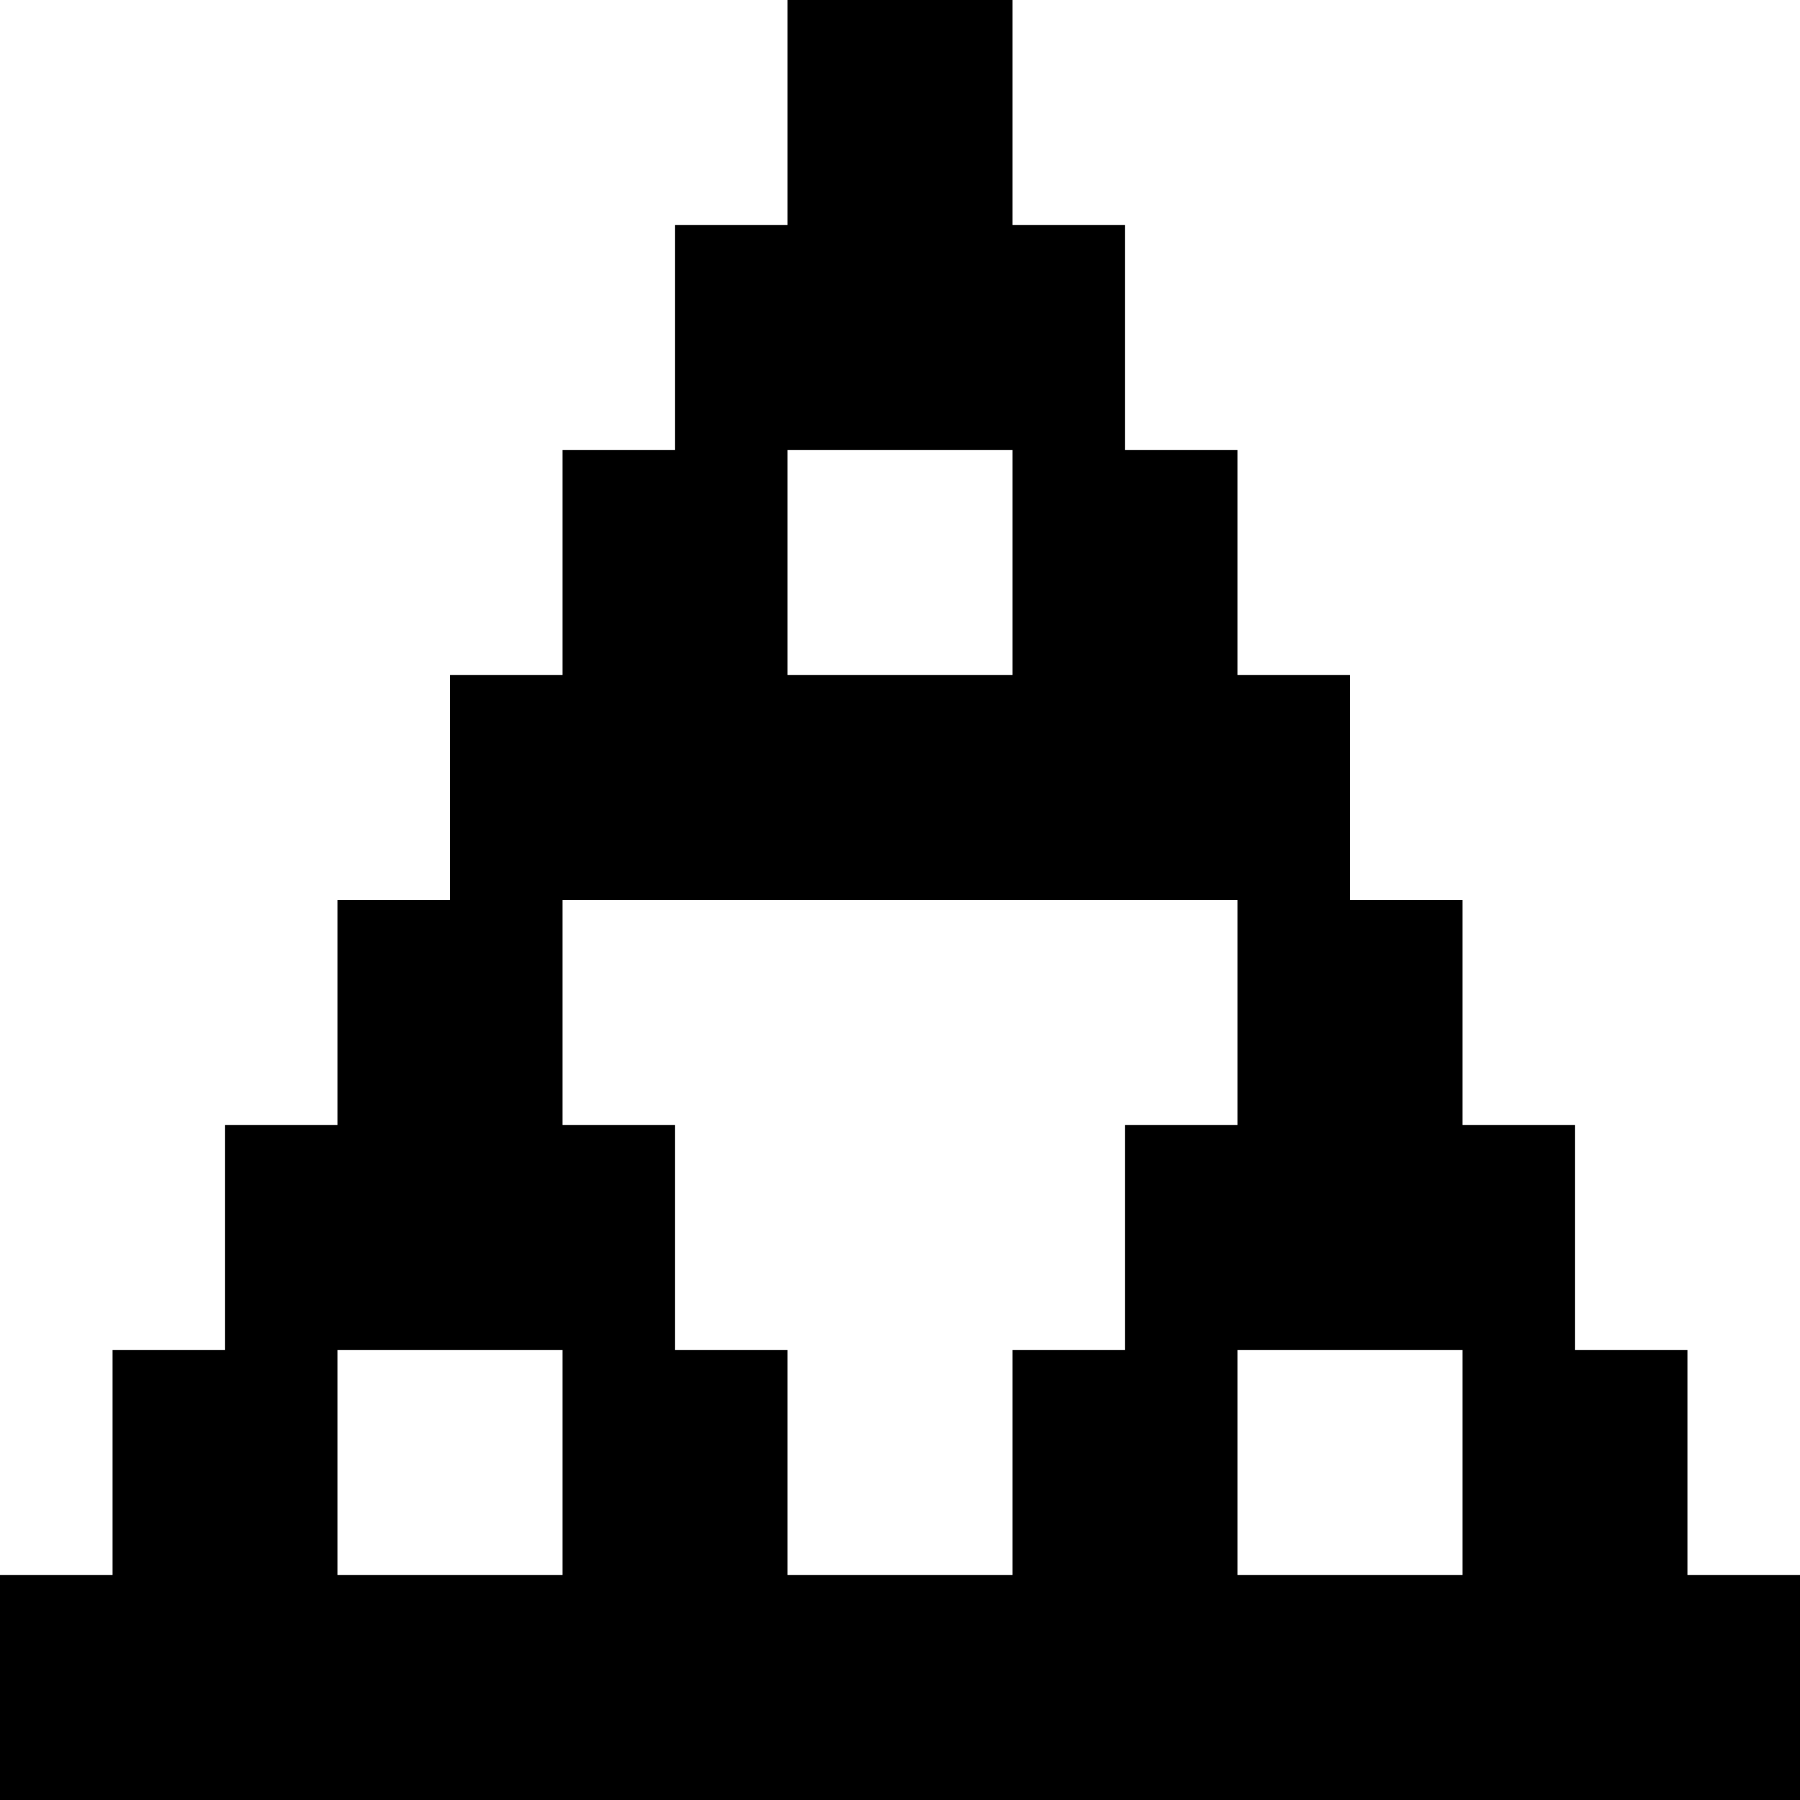
\includegraphics[width=0.25\textwidth]{papers/ifs/images/sierpinski3}}
	\subfigure[]{
		\label{ifs:sierpconstd}
		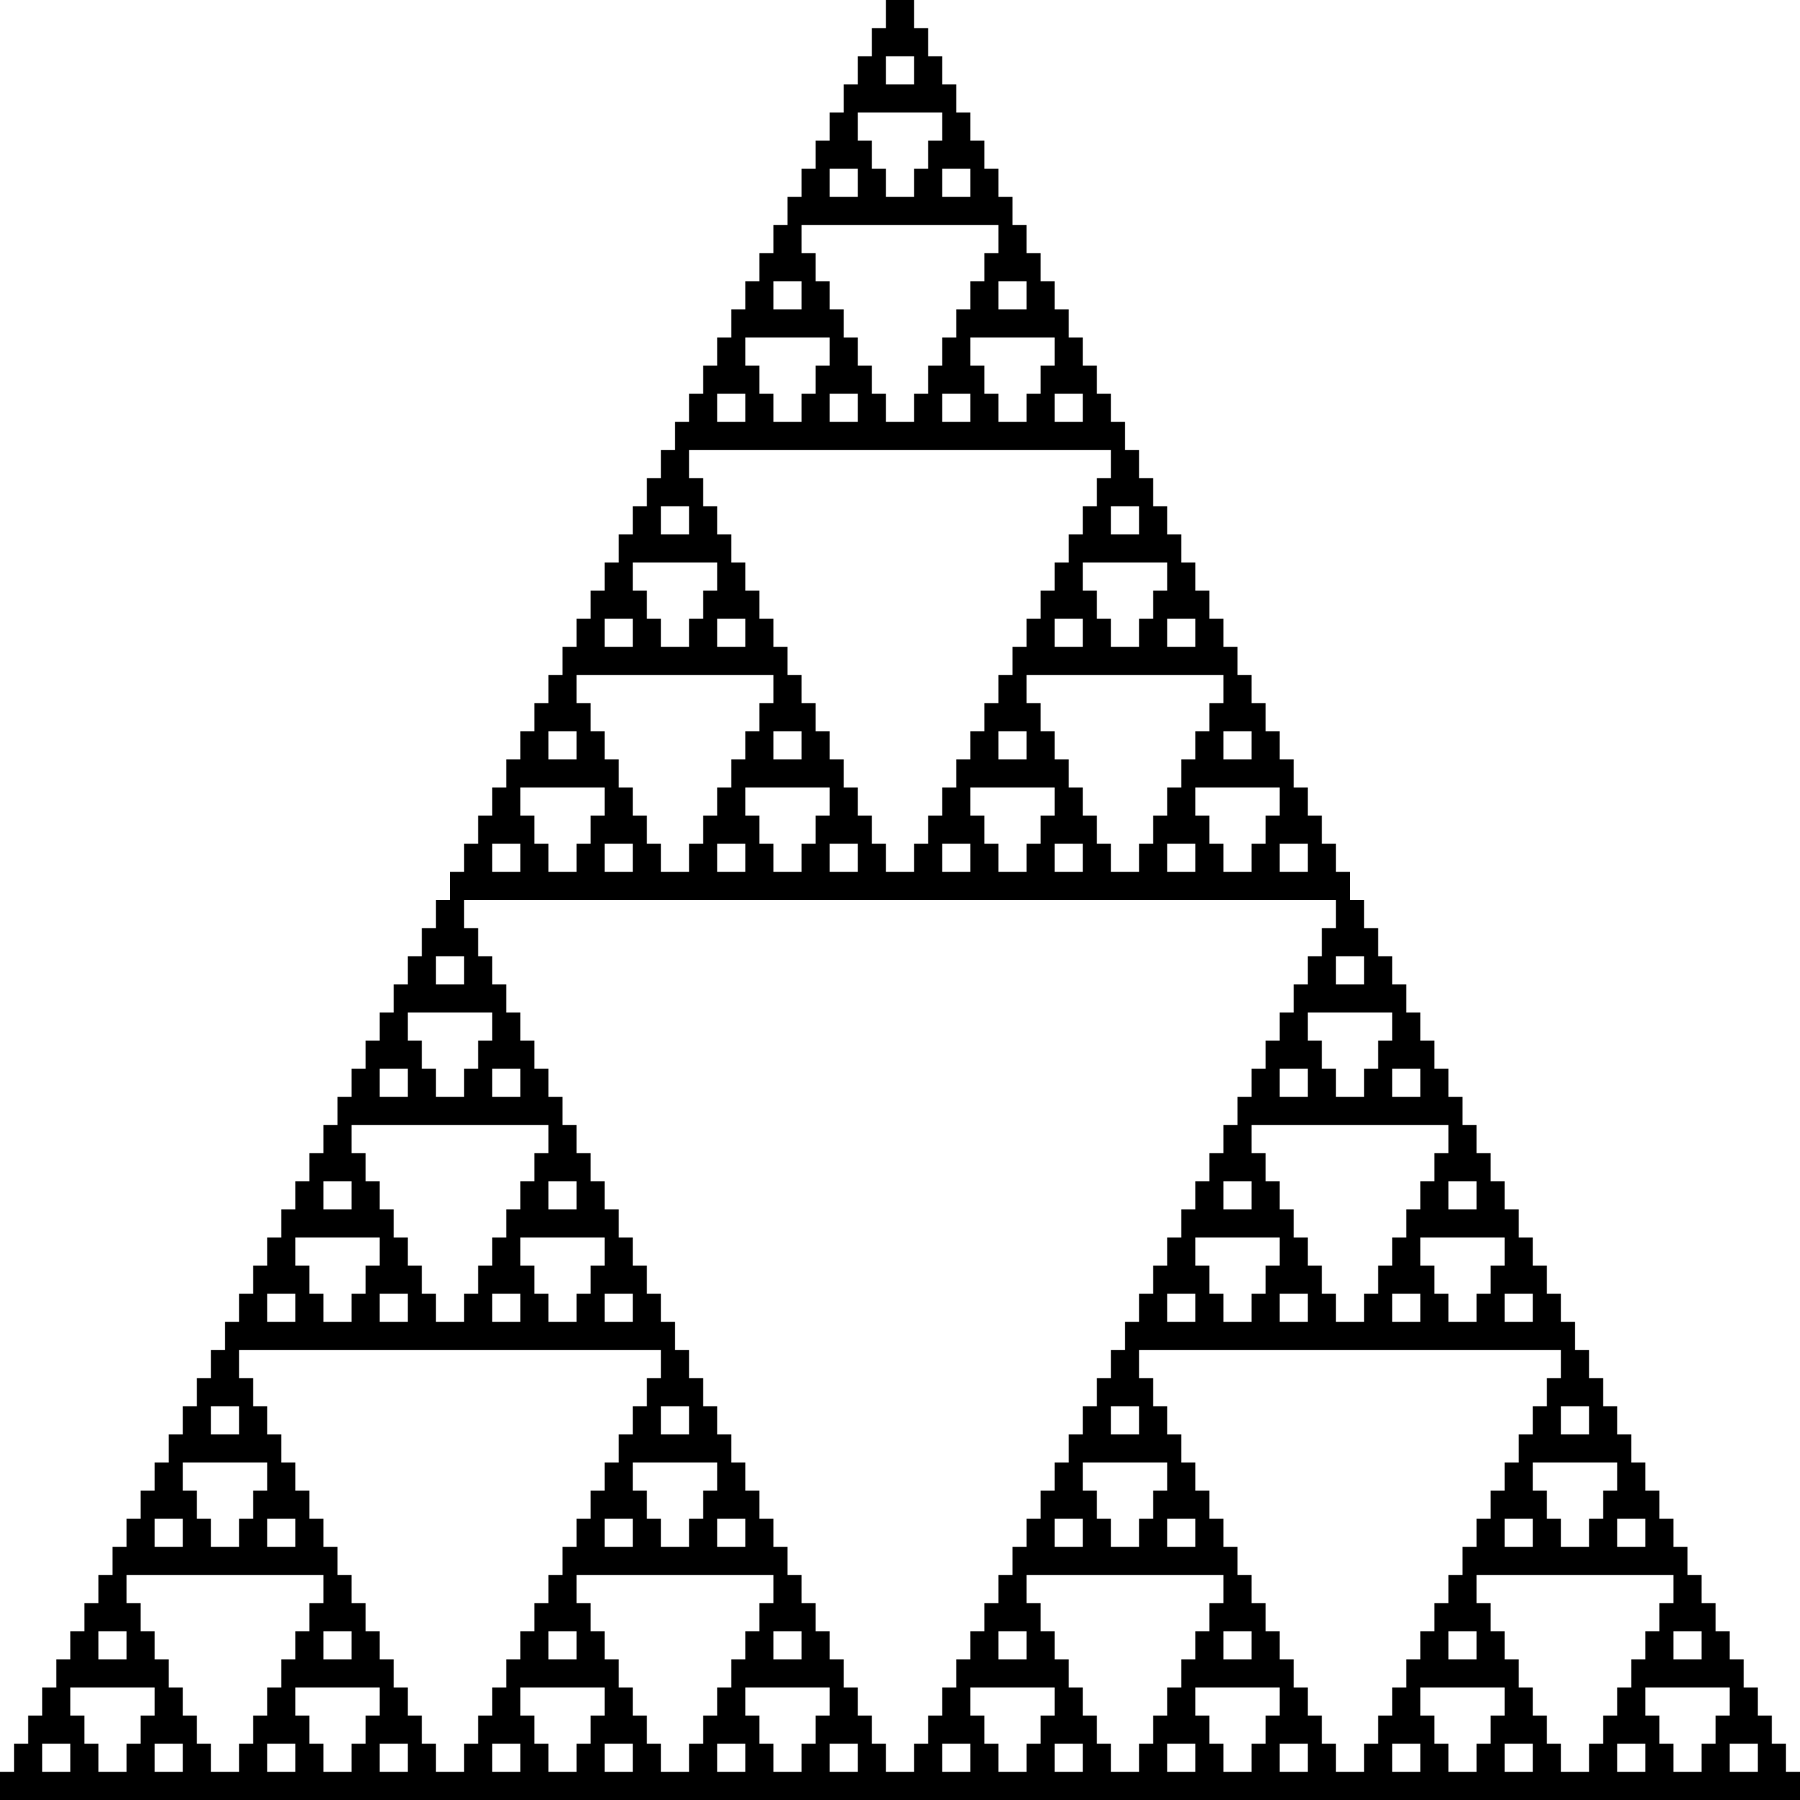
\includegraphics[width=0.25\textwidth]{papers/ifs/images/sierpinski6}}
	\caption{Konstruktion eines Sierpinski-Dreiecks mit einem Schwarzen Quadrat als Start\\
		(a) 1. Iteration (b) 2. Iteration (c) 3. Iteration (d) 5. Iteration}
\end{figure}
Im Beispiel der Abbildung \ref{ifs:sierpconst} sehen wir, wie das Bild nach jeder Iteration dem Sierpinski-Dreieck ähnlicher wird.
Der Abstand zum Original wird immer kleiner, und konvergiert bei unendlich Iterationen gegen null.

\subsection{Iterierte Funktionensysteme
\label{ifs:subsection:bonorum}}
In diesem Unterkapitel wollen wir die Erkenntnis, wie wir aus einer beliebigen Menge ein Sierpinski-Dreieck generieren können, verallgemeinern.
TODO TEXT

$S_1,...,S_n$ sind Kontraktionen auf die Menge $D \subset \mathbb{R}^n$. Es gilt
\begin{align}
	|S_i(x) - S_i(y)| \leq c_i|x - y|
\end{align}
für jedes i mit einem $c_i < 1$. Dann existiert eine eindeutige kompakte Menge $F$ für die gilt
\begin{equation}
	F = \bigcup\limits_{i = 1}^{m} S_i(F)
\end{equation}
TODO Text
